\documentclass{amsart}

\usepackage{../AMC_style}	
\usepackage{../Research}

\newcommand{\F}{\mathcal F}
\newcommand{\curly}[1]{\left\{ #1 \right\}}

%\DeclareMathOperator{\vc}{vc}

\begin{document}

\section{Combinatorics}

Suppose we have an infinite collection of sets $\F$.
Take $n$ many of those sets.
They generate a boolean algebra.
Count the number of atoms in it.
There can be at most $2^n$ atoms, though depending on the collection there may be much less.
For a given $n$, out of all choices of $n$ sets, record the highest possible number of atoms generated.
We define that to be a shatter function.

\begin{Definition}
	\begin{align*}
		\pi_\F(n) = \max \curly{ \text {\# of atoms in boolean algebra generated by $S$} \mid S \subset \F \text{ and } |S| = n}
	\end{align*}
\end{Definition}

Example: Let $\F$ consist of all discs in the plane.
\begin{figure}[p]
	\centering
	\includegraphics[scale=0.75]{circles.png}
\end{figure}
\begin{align*}
	\pi_\F(1) = 2 \ \ \  \pi_\F(2) = 4 \ \ \  \pi_\F(3) = 8  \ \ \ \pi_\F(4) = 14
\end{align*}
\begin{align*}
	\pi_\F(n) = n^2 - n + 2
\end{align*}

Example: Let $\F$ consist of all half-planes in the plane.
\begin{figure}[p]
	\centering
	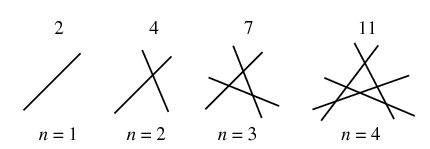
\includegraphics[scale=0.75]{lines.png}
\end{figure}
\begin{align*}
	\pi_\F(1) = 2 \ \ \  \pi_\F(2) = 4 \ \ \  \pi_\F(3) = 7  \ \ \ \pi_\F(4) = 11
\end{align*}
\begin{align*}
	\pi_\F(n) = n^2/2 + n/2 + 1
\end{align*}




\begin{Example}
	\begin{enumerate}
		\item Let $\F$ be a set of lines on a plane. Then
		\begin{align*}
			\pi_\F(n) &= n(n+1)/2 + 1
		\end{align*}
		\item Let $\F$ be a set of disks on a plane. Then
		\begin{align*}
			\pi_\F(n) &= n^2 - n + 2
		\end{align*}
		\item Let $\F$ be a set of balls in $\R^3$. Then
		\begin{align*}
			\pi_\F(n) &= n(n^2 - 3n + 8)/3
		\end{align*}
		\item Let $\F$ be a set of intervals on a line. Then
		\begin{align*}
			\pi_\F(n) &= 2n
		\end{align*}
		\item Let $\F$ be a set of half-planes. Then
		\begin{align*}
			\pi_\F(n) &= n(n+1)/2 + 1
		\end{align*}
		\item Let $\F$ be a collection of finite subsets of $\N$. Then
		\begin{align*}
			\pi_\F(n) &= 2^n
		\end{align*}
		\item Let $\F$ be a collection of polygons in a plane. Then
		\begin{align*}
			\pi_\F(n) &= 2^n
		\end{align*}
	\end{enumerate}
\end{Example}

\begin{Theorem} [Sauer-Shelah]
	Shatter function is either $2^n$ or bounded by a polynomial.
\end{Theorem}

\begin{Definition}
	Suppose growth of shatter function for $\F$ is polynomial.
	Let $r$ be the smallest real such that 
	\begin{align*}
		\pi_\F(n) = O(n^r)
	\end{align*}
	We define such $r$ to be the vc-density of $\F$.
	If shatter function grows exponentially, we let vc-density to be infinite.
\end{Definition}

\section{Model Theory}

Consider a structure with a language
\begin{align*}
	(\R, 0, 1, +, \cdot, \leq)
\end{align*}

We work with subsets of the underlying set definable by first-order formulas.
Those are called definable sets.

\begin{align*}
	\phi(x) &= 5 \leq x \leq 7.7 \vee x \leq 0\\
	\psi(x) &= \exists y \ y \cdot y = x \\
	\gamma(x) &= x \cdot x \cdot x \cdot x = 2 \\
\end{align*}

$\phi(\R)$ defines the set $[5, 7.7] \cup (-\infty, 0]$ in the structure above.
$\psi(\R)$ defines the set $[0, \infty)$ in the structure above.

\begin{enumerate}
	\item in rationals $(\Q, \cdot)$ $\gamma(x)$ defines an empty subset
	\item in reals $(\R, \cdot)$ $\gamma(x)$ defines a subset with two elements
	\item in complex numbers $(\C, \cdot)$ $\gamma(x)$ defines a subset with four elements
	\item in quaternions $(\mathbb H, \cdot)$ $\gamma(x)$ defines an infinite subset
\end{enumerate}

\begin{align*}
	\theta(x) = \forall y \exists z \ x \leq z \leq y
\end{align*}

\begin{enumerate}
	\item in $(\Q, \leq)$ $\theta(x)$ defines an empty subset
	\item in $(\N, \leq)$ $\theta(x)$ defines an empty subset
	\item in $(\Q^{\geq 0}, \leq)$ $\theta(x)$ defines the set $\{0\}$
\end{enumerate}

\begin{Definition}
	for a formula $\phi(x_1 \ldots x_n, y_1, \ldots y_m)$ we can plug in elements of our structure as parameters in places of $y$ variables. This gives us a collection of definable sets. 
\end{Definition}

\begin{Example}
	\begin{align*}
		\phi(x_1, x_2, y_1, y_2, y_3) = (x_1 - y_1)^2 + (x_2 - y_2)^2 \leq y_3^2
	\end{align*}
\end{Example}

In structure $(\R, +, \cdot, \leq)$ given $a,b,r \in \R$ the formula $\phi(x_1, x_2, a, b, r)$ defines a disk in $\R^2$ with radius $r$ with center $(a,b)$.

Thus all discs in $\R^2$ are defined uniformly by $\phi$.

What are the collection of sets we can consider when working with a model?

We can look at all definable subsets. That's not interesting, always has an infinite vc-density.
Uniformly definable families offer more interesting behavior.

A model is said to be NIP if all uniformly definable families have finite vc-density.

For a given model $M$, let $\vc$ function of $n$ to be the largest $\vc$-density achieved by $n$-dimensional families of uniformly definable sets.

\begin{align*}
	\vc_M(n) = max \curly{ \vc(\phi) \mid \phi(\vec x, \vec y) \text{ with } |\vec x| = n}
\end{align*}

It is easy to show that $\vc_M(n) \geq n$ for all models.

Open questions about vc functions.

Is $\vc_M(n) = n \vc_M(1)$? If not, is there a linear relationship?

\end{document}